% =====================================================================
%  Kollisionskaskaden -- Kurze Physik-Praesentation
%  Paul Kamm, TH Luebeck, betreut von Dr. Maurice Maurer
%
%  Bau:  pdflatex physik_praesentation.tex   (2x fuer Referenzen)
%
%  Videos (separate MP4-Dateien in videos/) werden ueber klickbare
%  Links gestartet -- in den meisten PDF-Viewern oeffnet das den
%  Systemplayer. Auf jeder Video-Folie liegt ein Standbild aus stills/.
% =====================================================================
\documentclass[aspectratio=169,11pt]{beamer}

\usetheme{metropolis}
\usepackage[ngerman]{babel}
\usepackage[utf8]{inputenc}
\usepackage[T1]{fontenc}
\usepackage{amsmath,amssymb}
\usepackage{graphicx}
\usepackage{booktabs}
\usepackage{multimedia}
\usepackage{tikz}

% --- Farben: tiefes Blau + warmes Orange (Kaskaden-Motiv) ------------
\definecolor{tiefblau}{RGB}{20,28,60}
\definecolor{glut}{RGB}{235,110,40}
\setbeamercolor{frametitle}{bg=tiefblau, fg=white}
\setbeamercolor{progress bar}{fg=glut}
\setbeamercolor{alerted text}{fg=glut}
\metroset{block=fill, numbering=fraction, progressbar=frametitle}

\graphicspath{{stills/}{figures/}{../results/images/}{./}}

% Bequemes Makro fuer eine Video-Folie: #1 Titel, #2 Standbild, #3 mp4, #4 Bildunterschrift
\newcommand{\videofolie}[4]{%
  \begin{frame}{#1}
    \centering
    \href{run:videos/#3}{\includegraphics[height=0.72\textheight]{#2}}\\[0.3em]
    {\footnotesize #4 \quad\alert{$\blacktriangleright$ \href{run:videos/#3}{Video abspielen}}}
  \end{frame}}

\title{Kollisionskaskaden}
\subtitle{Strahlenschaden in einem 2D-Modellkristall}
\author{Paul Kamm}
\institute{TH Lübeck \, ·\, betreut von Dr.\ Maurice Maurer}
\date{}

\begin{document}

\maketitle


% ---------------------------------------------------------------------
\begin{frame}{Das Modell}
  \begin{columns}[T]
    \begin{column}{0.54\textwidth}
      Atome auf einem \alert{Dreiecksgitter} (6 Nachbarn, schubstabil).
      Zwei Wechselwirkungen:
      \begin{itemize}
        \item \textbf{Brechbare Feder} $F=K(r-L_0)$,\\
          reißt bei 15\,\% Dehnung → \alert{Defekt}.
        \item \textbf{Steile Abstoßung} $\sim (R_\text{cut}/r)^{12}$,\\
          gibt Atomen einen Stoßquerschnitt.
      \end{itemize}
      \vspace{0.6em}
      Das PKA ist einfach ein Atom mit hoher Startgeschwindigkeit
      \[ v_\text{PKA}=\sqrt{2E_\text{PKA}/m}\;\gg\; c_\text{Schall}. \]
      Eine \alert{Hyperschall}-Kaskade.
    \end{column}
    \begin{column}{0.46\textwidth}
      \centering
      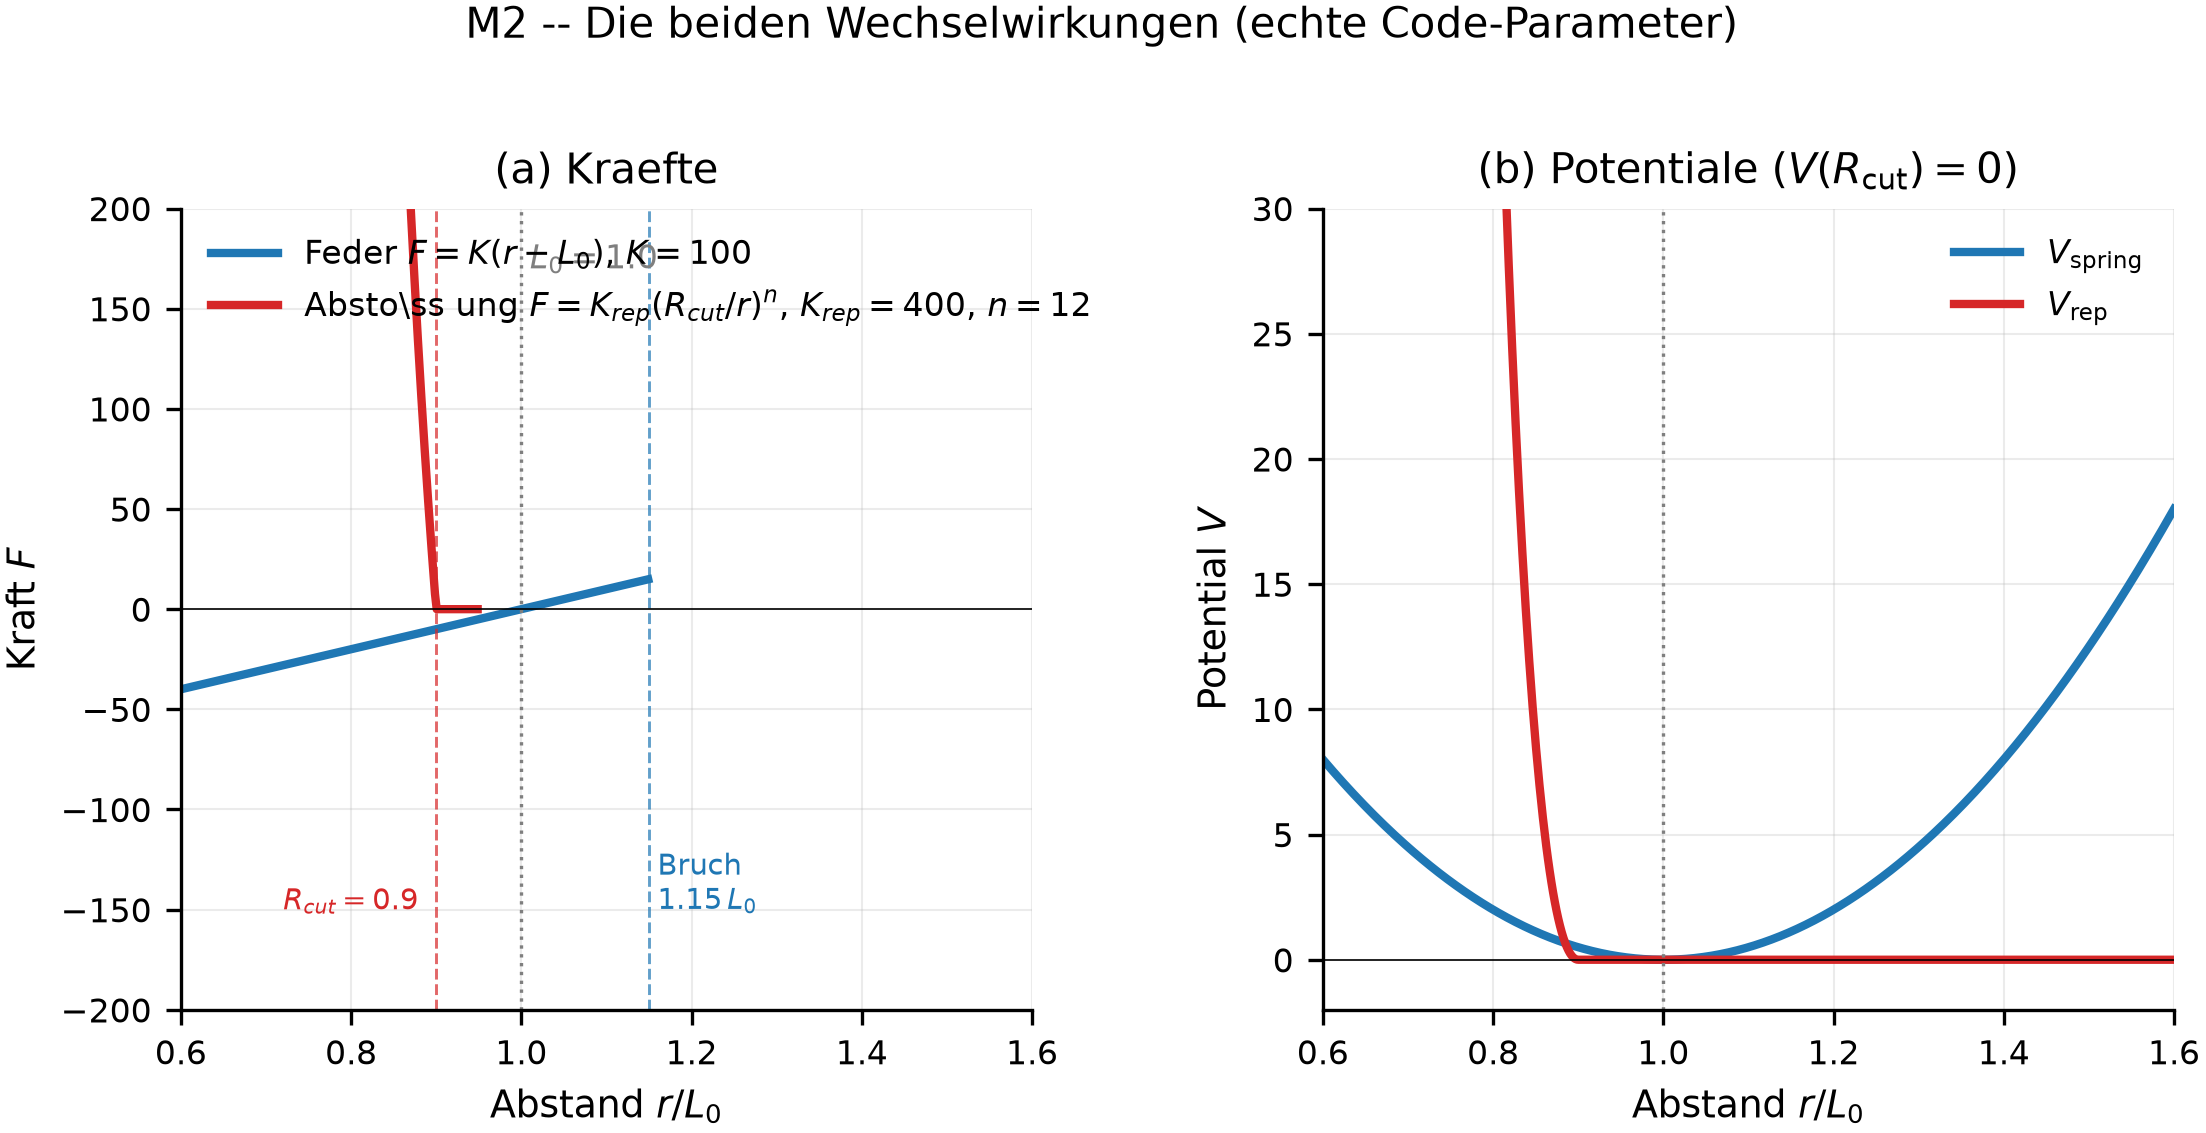
\includegraphics[width=\linewidth]{M2_force_law.png}\\
      {\scriptsize Die beiden Kräfte: Feder (blau) + Abstoßung (rot).}\\[0.5em]
      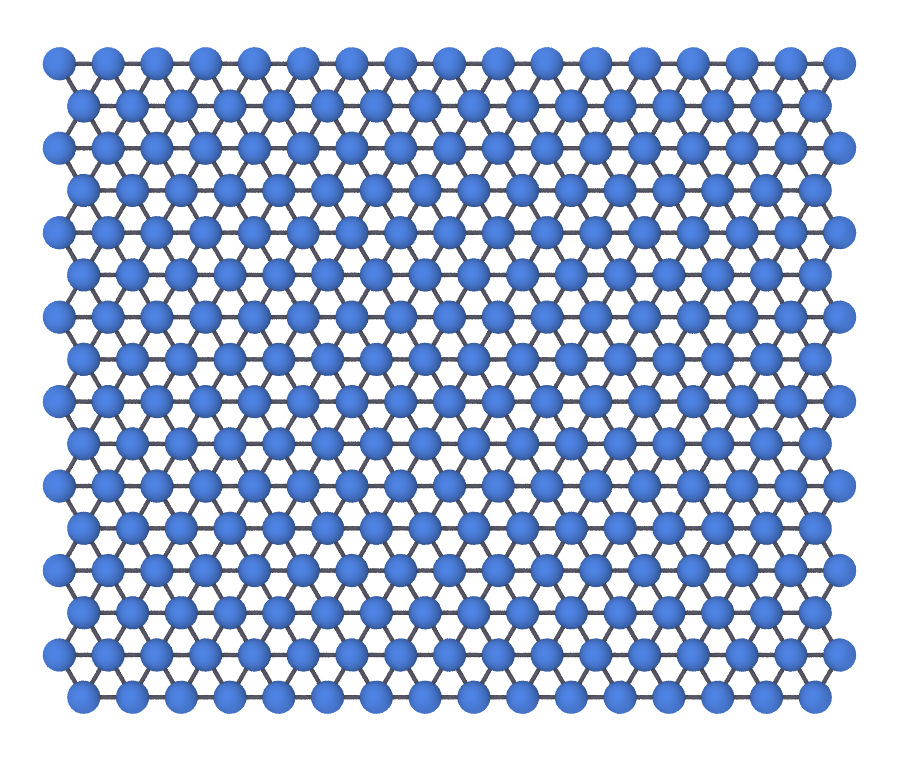
\includegraphics[width=0.6\linewidth]{modell_ruhelage.png}\\
      {\scriptsize Modell in Ruhelage: Dreiecksgitter mit Federbindungen.}
    \end{column}
  \end{columns}
\end{frame}

% ---------------------------------------------------------------------

\videofolie{1 · Der thermische Spike}{still_1.png}{cascade_1_geschwindigkeit.mp4}
  {Farbe = Geschwindigkeit. Die Einschlagsenergie wird zu einer heißen,
   ungeordneten Zone bewegter Atome, die expandiert und wieder abkühlt.}

\videofolie{2 · Die Schadensbildung}{still_2.png}{cascade_2_schaden.mp4}
  {Farbe = Zahl gerissener Bindungen. Die Defektstruktur wächst und
   \alert{friert} als bleibender Cluster ins Gitter ein.}

\videofolie{3 · Das Verschiebungsfeld}{still_3.png}{cascade_3_verschiebung.mp4}
  {Farbe = bleibende Auslenkung vom Gitterplatz. Sichtbar wird der
   „Heat-Spike``: eine kompakte Zone dauerhaft verschobener Atome.}

\videofolie{4 · Reale Bestrahlung: viele Einschläge}{still_4.png}{cascade_4_mehrere_pka.mp4}
  {Fünf gleichzeitige PKAs. Überlappende Kaskaden -- und ein Atom, das
   entlang einer Gitterrichtung \alert{kanalisiert} (der lange Track).}

% ---------------------------------------------------------------------
\begin{frame}{Das physikalische Ergebnis: ein Potenzgesetz}
  \begin{columns}[T]
    \begin{column}{0.52\textwidth}
      Über \alert{1000 Kaskaden} gemittelt folgt die Verteilung der
      Clustergrößen einem Potenzgesetz:
      \[ F(n)\;\propto\; n^{-S},\qquad S \approx 1{,}4. \]
      \begin{itemize}
        \item \alert{Skalenfrei}: keine „typische`` Clustergröße --
          Kennzeichen selbstorganisierter Kritikalität.
        \item \alert{Robust}: mit/ohne Defektheilung fast identisch
          ($S=1{,}36$ vs.\ $1{,}39$).
        \item Vergleich 3D-Wolfram (Sand et al.\ 2013): $S=1{,}63$.
          Der 2D-Wert liegt konsistent darunter.
      \end{itemize}
    \end{column}
    \begin{column}{0.48\textwidth}
      \centering
      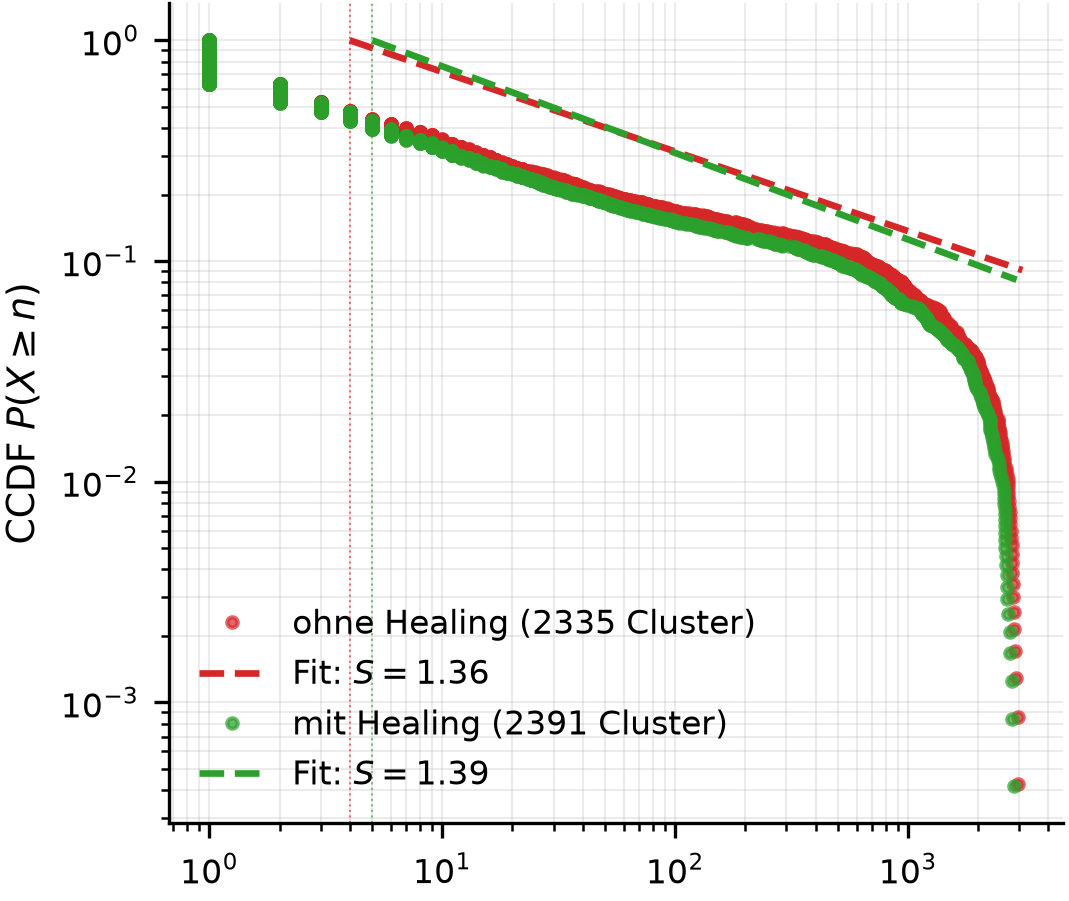
\includegraphics[width=\linewidth]{powerlaw_ccdf.png}\\
      {\scriptsize CCDF über Clustergröße $n$ (log-log): eine Gerade über
       fast drei Größenordnungen.}
    \end{column}
  \end{columns}
\end{frame}


\end{document}
